\chapter{Discussion}
\label{chap:discussion}
\paragraph{\textnormal{This chapter presents interpretation of the results obtained from the experiments, highlighting the strengths and limitations of the proposed hybrid LiDAR SLAM framework. The discussion connects the findings with the original research objectives, evaluates their implications in both indoor and outdoor scenarios, and reflects on how the integration of FAST-LIO2, loop closure with Scan Context and factor graph, and bundle adjustment contributed to global consistency. Furthermore, it explores the challenges encountered during implementation and analysis, providing insights that can inform future enhancements and deployments of SLAM systems in complex environments.}}

\section{Interpreting the results}
\paragraph{\textnormal{The experimental results demonstrate the effectiveness of the proposed hybrid LiDAR SLAM pipeline in achieving globally consistent mapping across diverse indoor and outdoor environments. The trajectory accuracy and map consistency metrics reveal that integrating FAST-LIO2 with PGO significantly reduces accumulated drift compared to using FAST-LIO2. Moreover, applying HBA on top of PGO optimized map further refines the global consistency of the map.
}}

%\paragraph{\textnormal{As shown in Table \ref{tab:traj_error_saxion}, the APE of translation for Saxion-01 decreases from 6.33 m with FAST-LIO2 to 2.51 m after applying PGO. Similarly, Figure \ref{fig:saxion01_map} shows the misaligned FAST-LIO2 map with \textbf{10m} vertical gap (Figure \ref{fig:saxion01_traj}c) in the revisited area which is corrected after applying PGO as shown in Figure \ref{fig:saxion01_map}d. Even after PGO optimization, Figure \ref{fig:saxion01_map}b and Figure~\ref{fig:kaist3_map}e, we still see misalignment and duplication in the map. This is due to the fact that PGO does not globally optimize the point cloud consistency. Additionally, errors in loop closure using ICP also count to these inconsistencies. Applying HBA on top of this map results in more consistent map as shown in Figure \ref{fig:saxion01_map}e. The For \texttt{saxion02}, the APE of translation increased from \textbf{3.71~m} to \textbf{4.04~m} due to limited loop closures and a \textbf{15~m} lateral shift in the revisited area, where loop detection failed. Although radius search was used to compensate for the failure in Scan Context, ICP alignment introduced errors, worsening map and trajectory consistency. \texttt{Saxion03} has relatively more loop closures and multiple revisited areas and the PGO significantly improved map quality and trajectory accuracy. In \texttt{Saxion-11}, FAST-LIO2 shows minimal drift because indoor environment (see Figure~\ref{fig:saxion_indoor}) has structured geometrical primitives (edges, and planes) providing strong and stable constraints for scan registration. }}
%
%\paragraph{\textnormal{ MME score of the maps generated by each mapping component for all datasets is shown in Table~\ref{tab:mme}. The results show effective correction of drift via loop closure further improving the accuracy by refining global consistency.}}
\subsection{Trajectory and Map Accuracy}
\paragraph{\textnormal{
		As shown in Table~\ref{tab:traj_error_saxion}, the APE of the translation for \texttt{Saxion-01} decreases from 6.33~m with FAST-LIO2 to 2.51~m after applying PGO. Figure~\ref{fig:saxion01_map} illustrates this correction, where a vertical misalignment of about 10~m in the revisited area (Figure~\textcolor{blue}{\ref{fig:saxion01_traj}c}) is corrected after PGO (Figure~\textcolor{blue}{\ref{fig:saxion01_map}d}). However, residual misalignments remain after PGO (Figure~\textcolor{blue}{\ref{fig:saxion01_map}b} and Figure~\textcolor{blue}{\ref{fig:kaist3_map}e}), due to ICP inaccuracies and the fact that PGO does not globally optimize point cloud consistency. Applying HBA further refines the map, resulting in a more consistent reconstruction (Figure~\textcolor{blue}{\ref{fig:saxion01_map}e}).
}}

\paragraph{\textnormal{
		For \texttt{Saxion-02}, the APE increases slightly from 3.71~m to 4.04~m due to limited loop closures and a 15~m lateral shift in the revisited area, which caused loop detection to fail. Although radius-based search was used to compensate for Scan Context’s failure, ICP introduced alignment errors. In contrast, \texttt{Saxion-03} has multiple revisited areas, and the use of PGO and HBA significantly improved both trajectory accuracy and map quality.
}}

\paragraph{\textnormal{
		In \texttt{Saxion-11}, FAST-LIO2 alone performs well with minimal drift, as the structured indoor environment (Figure~\ref{fig:saxion_indoor}) contains abundant geometric features like edges and planes, providing strong constraints for scan registration.
}}

\paragraph{\textnormal{
		The MME scores in Table~\ref{tab:mme} confirm that PGO and HBA significantly improve map quality across all datasets by enhancing global consistency. The only exception is the indoor \texttt{Saxion-11}, where FAST-LIO2 already produces a consistent map (Figure~\ref{fig:saxion_indoor}) due to the structured environment, leaving little room for further improvement.
}}

\subsection{Discussing the ATE and MME comparison results}
\paragraph{\textnormal{
		Table~\ref{tab:traj_error_public_comp} presents the RMSE of the trajectories of the proposed method and other SOTA SLAM methods for the three public datasets. The RMSE of the pair of trajectories is computed after they are aligned using Umeyama algorithm in Evo. The best-performing method for each dataset is highlighted in bold. For the \texttt{KITTI05} dataset, MOLA achieves the lowest error at \textbf{1.80m} and the proposed method achieves \textbf{2.80m}. For \texttt{ KAIST03} dataset, the proposed method outperforms the other methods with an error of \textbf{2.42m}, significantly lower than the other methods. It is important to note that KISS SLAM results were not aligned due to missing timestamps in its outputs, leading to high errors and an overly optimistic comparison. Similarly, for the \texttt{KITTI00} dataset, the proposed method performs best with RMSE of \textbf{2.55m}.
}}

\paragraph{\textnormal{Figure~\ref{fig:sota_comp_traj} provides a detailed visual comparison of the of the APE, complementing the RMSE summary in Table~\ref{tab:traj_error_public_comp}. The Figures~\ref{sub_fig:ki0_err}, \ref{sub_fig:ka3_err}, and \ref{sub_fig:ki5_err} shows the APE over time computed for the entire trajectory of KITTI00, KAIST03, and KITTI05 respectively. Overall, proposed method demonstrated better performance indicating its potential for reliable  pose estimation across different scenarios.
}}

\paragraph{\textnormal{
Table \ref{tab:sota_mme} presents the  MME comparison of the proposed method and other SLAM methods across the datasets. The proposed method consistently achieves either the best or second-best results in all sequences, indicating superior or comparable map quality. Notably, it outperforms other methods in five out of seven cases, demonstrating its effectiveness in generating accurate and consistent map both for indoor and outdoor environments.
}}

\section{Challenges}
\paragraph{\textnormal{ One of the primary challenges faced was the failure in loop closure detection when a place is revisited in a reverse direction or there is a lane-level lateral shift in revisiting a place, see Figure~\ref{fig:lcd_failure}. This issue was exacerbated when the horizontal FoV of the LiDAR is partially occluded or unavailable, leading to a complete failure in loop detection. As a fallback, a radius based search was employed to identify potential loop candidates from which the one with smallest registration error was chosen as a loop. However, subsequent ICP registration often yielded inaccurate alignment and even sometimes introducing false positives due to inefficiency of the radius-based search.
}}

\paragraph{\textnormal{
Another critical challenge was the occurrence of false positive loop closures in environments with repetitive structures such as greenhouses, and bridges presented similar features over long stretches. This makes it difficult for the loop detection algorithm to distinguish between truly revisited locations and visually similar but distinct areas. These false matches led to incorrect loop closures, compromising the overall map consistency. Figure~\ref{fig:grnhs_pgo} shows the effect of such false loop closures in consistency of the map.
}}

\begin{figure}[H]
	\centering
	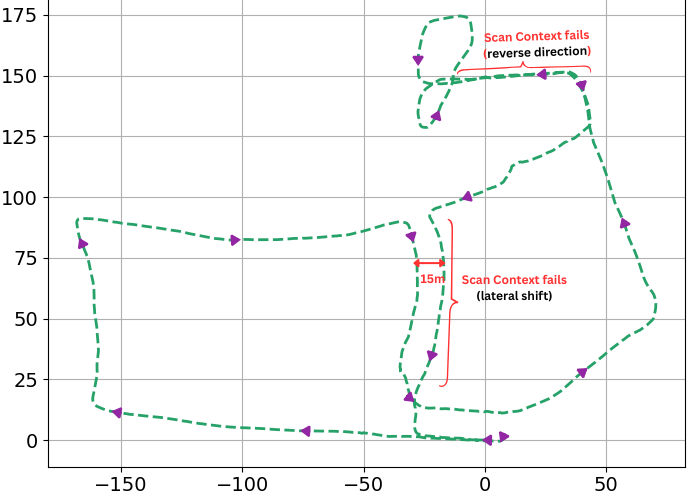
\includegraphics[height=0.5\textwidth]{images/challenge.png}
	\caption{Loop detection failure case in lane-level later shift and reverse revisit}
	\label{fig:lcd_failure}
\end{figure}

\begin{figure}[H]

		\centering
		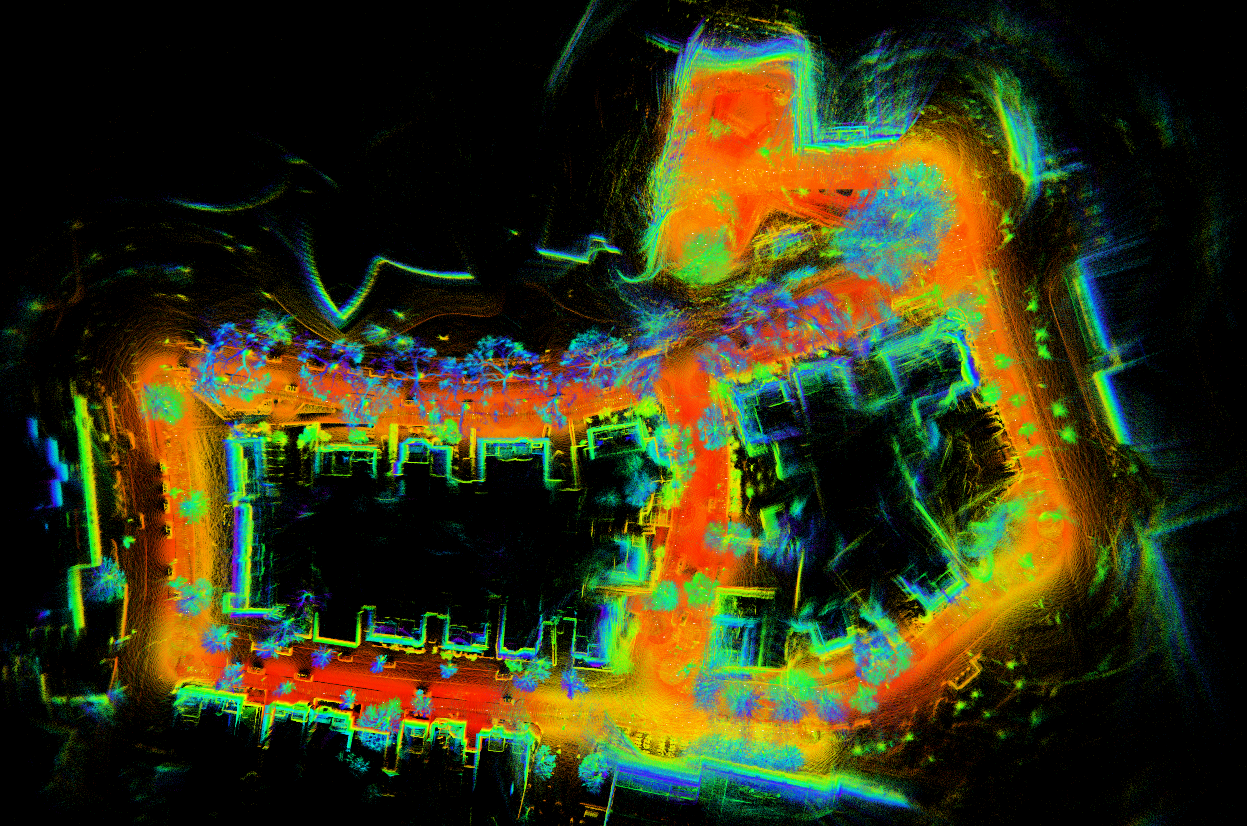
\includegraphics[width=0.8\textwidth]{images/challeng_map.png}
		\caption{}\caption{Effect of loop detection failure in the map}
	\label{fig:lcd_failure_map}
\end{figure}